\documentclass[11pt, oneside]{article}   	
\usepackage{geometry}                		
\geometry{letterpaper, margin=1in}              
\usepackage{graphicx}					
\usepackage{amssymb}
\usepackage{amsmath}
\usepackage{booktabs}
\usepackage{listings}
\usepackage{color}
\usepackage{multirow}
\usepackage{siunitx}
\usepackage[ruled,vlined]{algorithm2e}

\definecolor{dkgreen}{rgb}{0,0.6,0}
\definecolor{gray}{rgb}{0.5,0.5,0.5}
\definecolor{mauve}{rgb}{0.58,0,0.82}

\lstset{frame=tb,
   language=[90]Fortran,
   aboveskip=3mm,
   belowskip=3mm,
   showstringspaces=false,
   columns=flexible,
   basicstyle={\small\ttfamily},
   numbers=none,
   numberstyle=\tiny\color{gray},
   keywordstyle=\color{blue},
   commentstyle=\color{dkgreen},
   stringstyle=\color{mauve},
   breaklines=true,
   breakatwhitespace=true
   tabsize=3
   }


\title{MCSC 6030G : High Performance Computing \\ Assignment 4: Random Matrices with MPI}
\author{Parikshit Bajpai \\ 100693928}
\date{}							% Activate to display a given date or no date

\begin{document}
\maketitle

\section{Introduction}
This study is aimed at implementing the master-slave MPI model for computing maximum Eigenvalues of random matrices and finding the distribution of the Eigenvalues for a large number of matrices.

For a symmetric matrix $A [ n \times n]$, with elements normally distributed according to eqn~\ref{Eq1}, the Eigenvalues for any solution toare defined as the solution to the Eigenvalue problem $\mathbf{A}\mathbf{v}=\lambda \mathbf{v}$, where the vector $\mathbf{v}$ is called as the Eigenvector.

\begin{equation} \label{Eq1}
A_{ii} \sim N(0,2)(1\leq i\leq n) \quad\text{}\quad
A_{ij} \sim N(0,1)(1\leq i\leq j\leq n) \quad\text{}\quad
A^{t}=A
\end{equation}

For a random matrix $A$, the maximum the Eigenvalues, $\lambda _{max}$ should be a random number and the distribution of such maximum Eigenvalues can be determined. 

\section{Methodology}
   \subsection{Objective}
In the present assignment, the aforementioned distribution of maximum Eigenvalues has been computed for large matrices using master-slave MPI model and the speed-up and efficiency of parallelization has been examined.


\subsection{Machine Configuration}
The initial computations for the present study were performed on the local machine with the following specifications:
      \subsubsection{Local Machine}
        \textbf{Manufacturer}: Asus\\
	\textbf{Processor}: Intel Core i7 -7700HQ (4 physical cores, 4 hyperthreads)\\
	\textbf{RAM}:  16 GB\\
	\textbf{Operating System}: Ubuntu 18.04\\


	
\subsection{Implementation}
The master-slave model was implemented for the present study with the master tasked with keeping a track of the numbver of computations performed, receiving and collecting the outputs computed by each slave, and issuing instructions for the ideal slaves. Each of the slaves is tasked with generating a random matrix, computing the maximum Eigenvalue and sending the results back to the master. The pseudo code explaining the adopted methodology is as follows: 

\begin{algorithm}
Size of matrices $(n)$\\
Number of maximum eigenvalues to be collect ($\lambda _{max}$) $(Ni)$ \\
Set $\textit{flag}=1$, which means that slaves can continue working \\
Set $\textit{jobcount}=0$, which means that master did not receive any $\lambda _{max}$ so far\\
Start implementation Master vs Slave method\\~\\

\uIf{\text{PROC = SLAVE}}{
	Call MKL (Math Kernel Library) to Generate matrix randomly following normal distribution $N(0,1)$\\
	Make $A$ symmetric and multiply its diagonal by 2 ($2*A(n,n)$), adjusting matrix to problem proposed\\
	Calculate vector $W$ of eigenvalues (Using Lapack or Power Method)\\
	Define $\lambda _{max} = \text{max}(\lambda _{i})$ of vector $W$\\
	Call mpi and \textit{SEND} $\lambda _{max}$ to Master\\
	Call mpi and \textit{RECEIVE} $flag$ to verify if is there any job left\\
}
\textbf{end if} \\

\uIf{\text{PROC = MASTER}}{
		Define and allocate $G$ as a vector to store all $\lambda _{max}$ to be received from slaves\\
		Set $ith=1$, which is the position at vector $G$ that $\lambda _{max}$  to be receive will be allocated\\		
		\While{$ith < Ni$}{
			Call MPI and \textit{RECEIVE} $\lambda _{max}$ from slaves ($proc_i$)\\
			Increment $jobcount=jobcount+1$\\
			\uIf{$\textit{jobcount}$ $\leq$ $(Ni-\text{Numproc}+1)$}{
			$flag = 1$\\
			Call MPI and \textit{SEND} $flag$ to ($proc$) that hand in the $\lambda _{max}$ at that point\\
			\Else{
			$flag = 0$\\
			Call MPI and \textit{SEND} $flag$ to ($proc$) that hand in the $\lambda _{max}$ at that point
			}
			}
			Increment $ith=ith+1$\\
		\textbf{end if} \\	
		\textbf{end do} \\
		}  	
}	
\textbf{end if} \\
\caption{MAIN PROGRAM}
\label{algomain}
\end{algorithm}

For the implementation of the above code, the random numbers were seeded using the Marsenne Twister pseudorandom number generator included in the Intel Math Kernel Library (MKL). For computing the maximum eigenvalues, both the shifted power iterations and the LAPACK subroutine \emph{dsyev} were implemented. The LAPACK subroutine is a $\mathcal{O}(n^3)$ while the power iteartion is a $\mathcal{O}(n^2)$ method. While this means the power method is normally much quicker, there can be issues related to convergence especially if the Eigenvalues are very close. Furthermore, the compute time in the power iteration would also depend on the initial approximation of the Eigenvector.

\subsection{Computational Experiments}
The following studies were performed as part of this experiment:
\begin{enumerate}
\item Analyze the random distribution of the maximum Eigenvalues for different matrix sizes and different desired number of Eigenvalues.
\item Compare wallclock times for LAPACK subroutines and shifted power method.
\item Compare wallclock times for different number of processors.
\end{enumerate}

	
\section{Results and Discussion}
The obtained frequency distribution for a matrix of size $1000 \times 1000$ for $1000$ matrices has been shown below in figure~\ref{fig:dist}
 \begin{figure}[h]
		\centering
		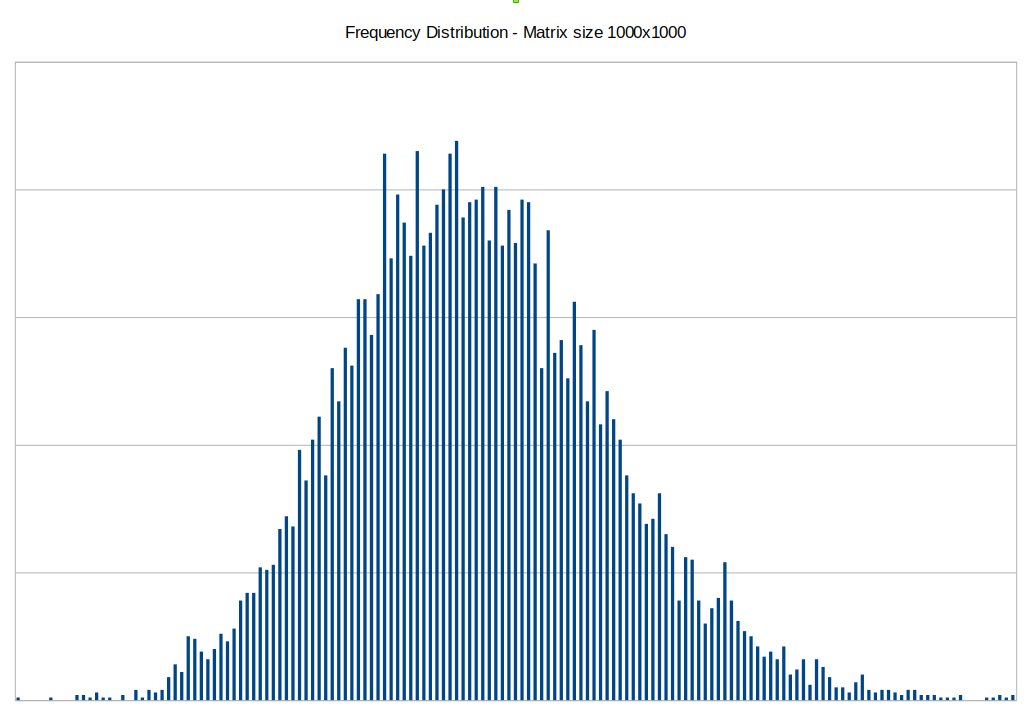
\includegraphics[width=0.75\textwidth]{Figures/n1000.png}
		\caption{Distribution of maximum Eigenvalues for a matrix of size $1000 \times 1000$ for $1000$ matrices.}
		\label{fig:dist}
	\end{figure}

The obtained random distributions of maximum Eigenvalues for different matrix sizes $n$ and different numbers of desired Eigenvalues $N$ using both BLAS and shifted power iterations for different matrix sizes are presented in figures~\ref{fig:1}~\&~\ref{fig:2}.
        \begin{figure}[h]
		\centering
		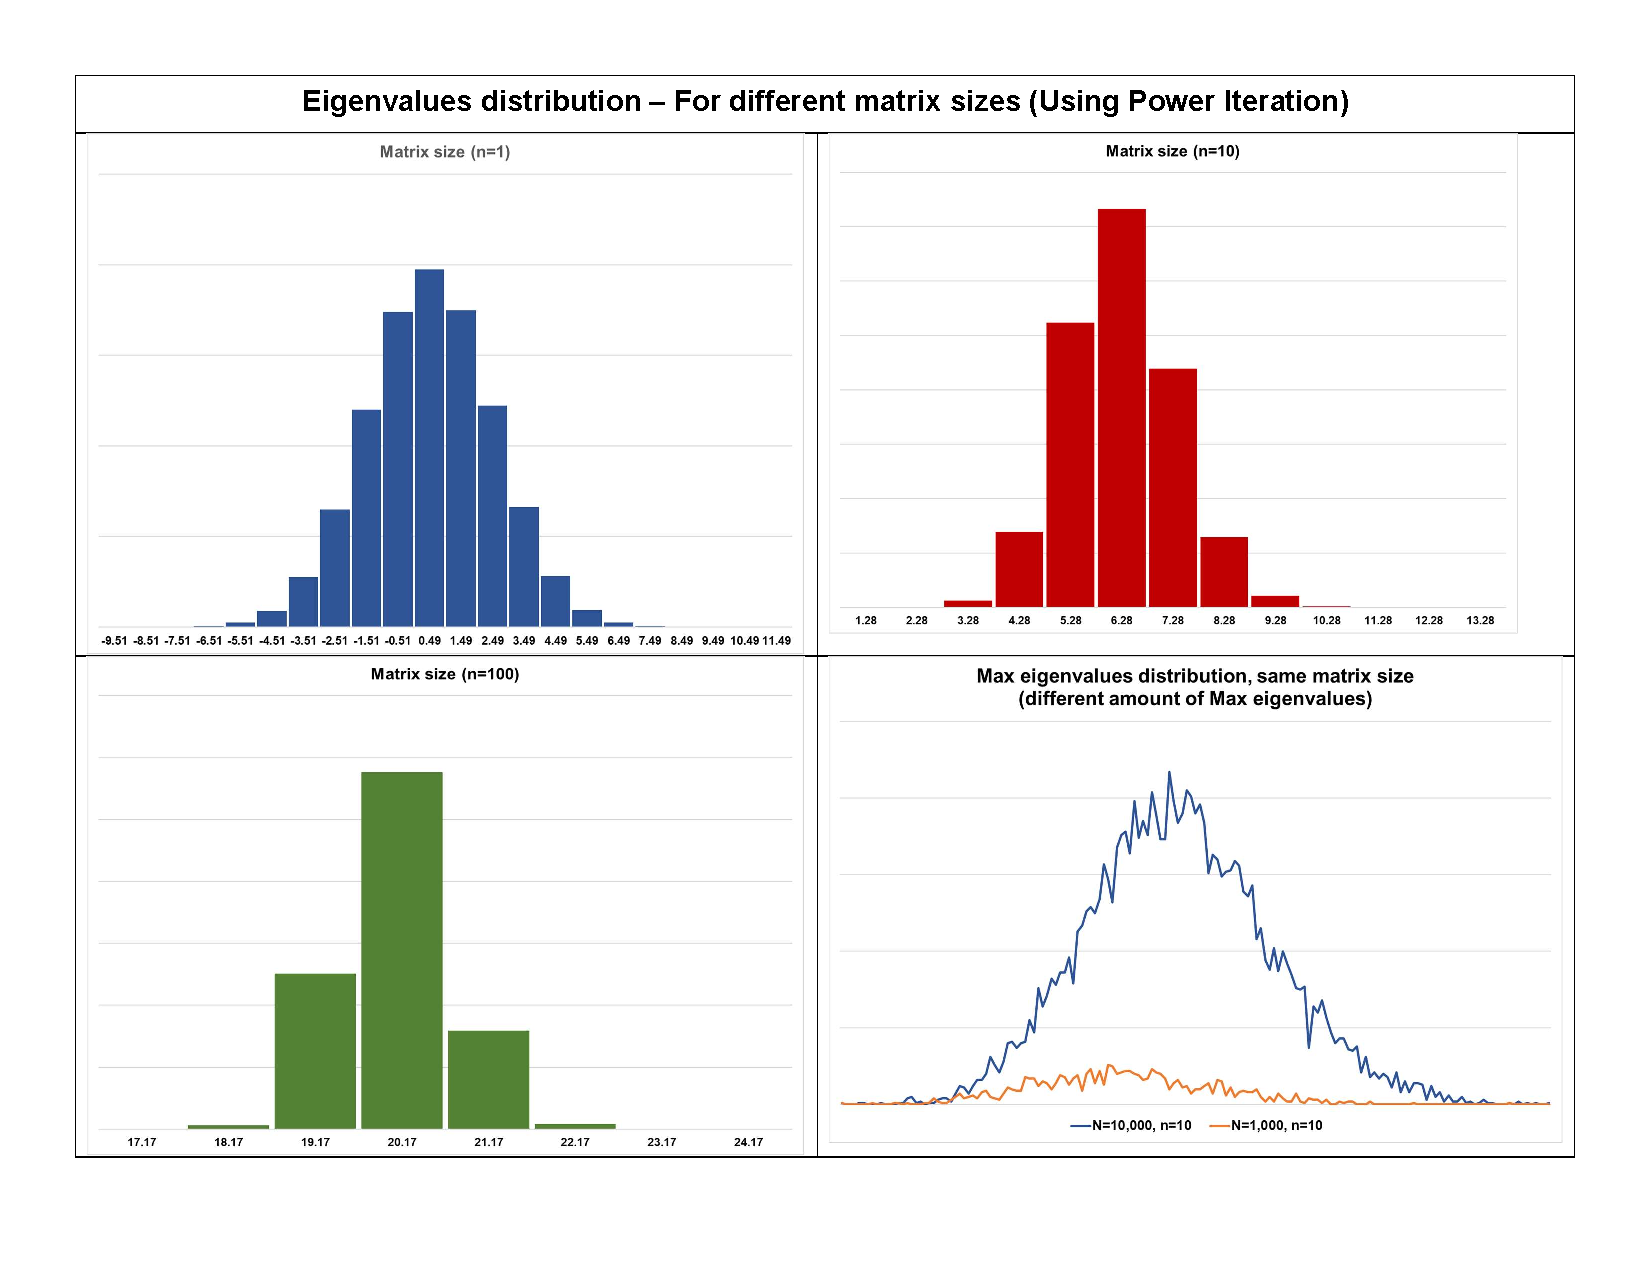
\includegraphics[width=0.75\textwidth]{Figures/D_power.pdf}
		\caption{Distribution of maximum Eigenvalues for computations using shifted power iterations.}
		\label{fig:1}
	\end{figure}
	\begin{figure}[h]
		\centering
		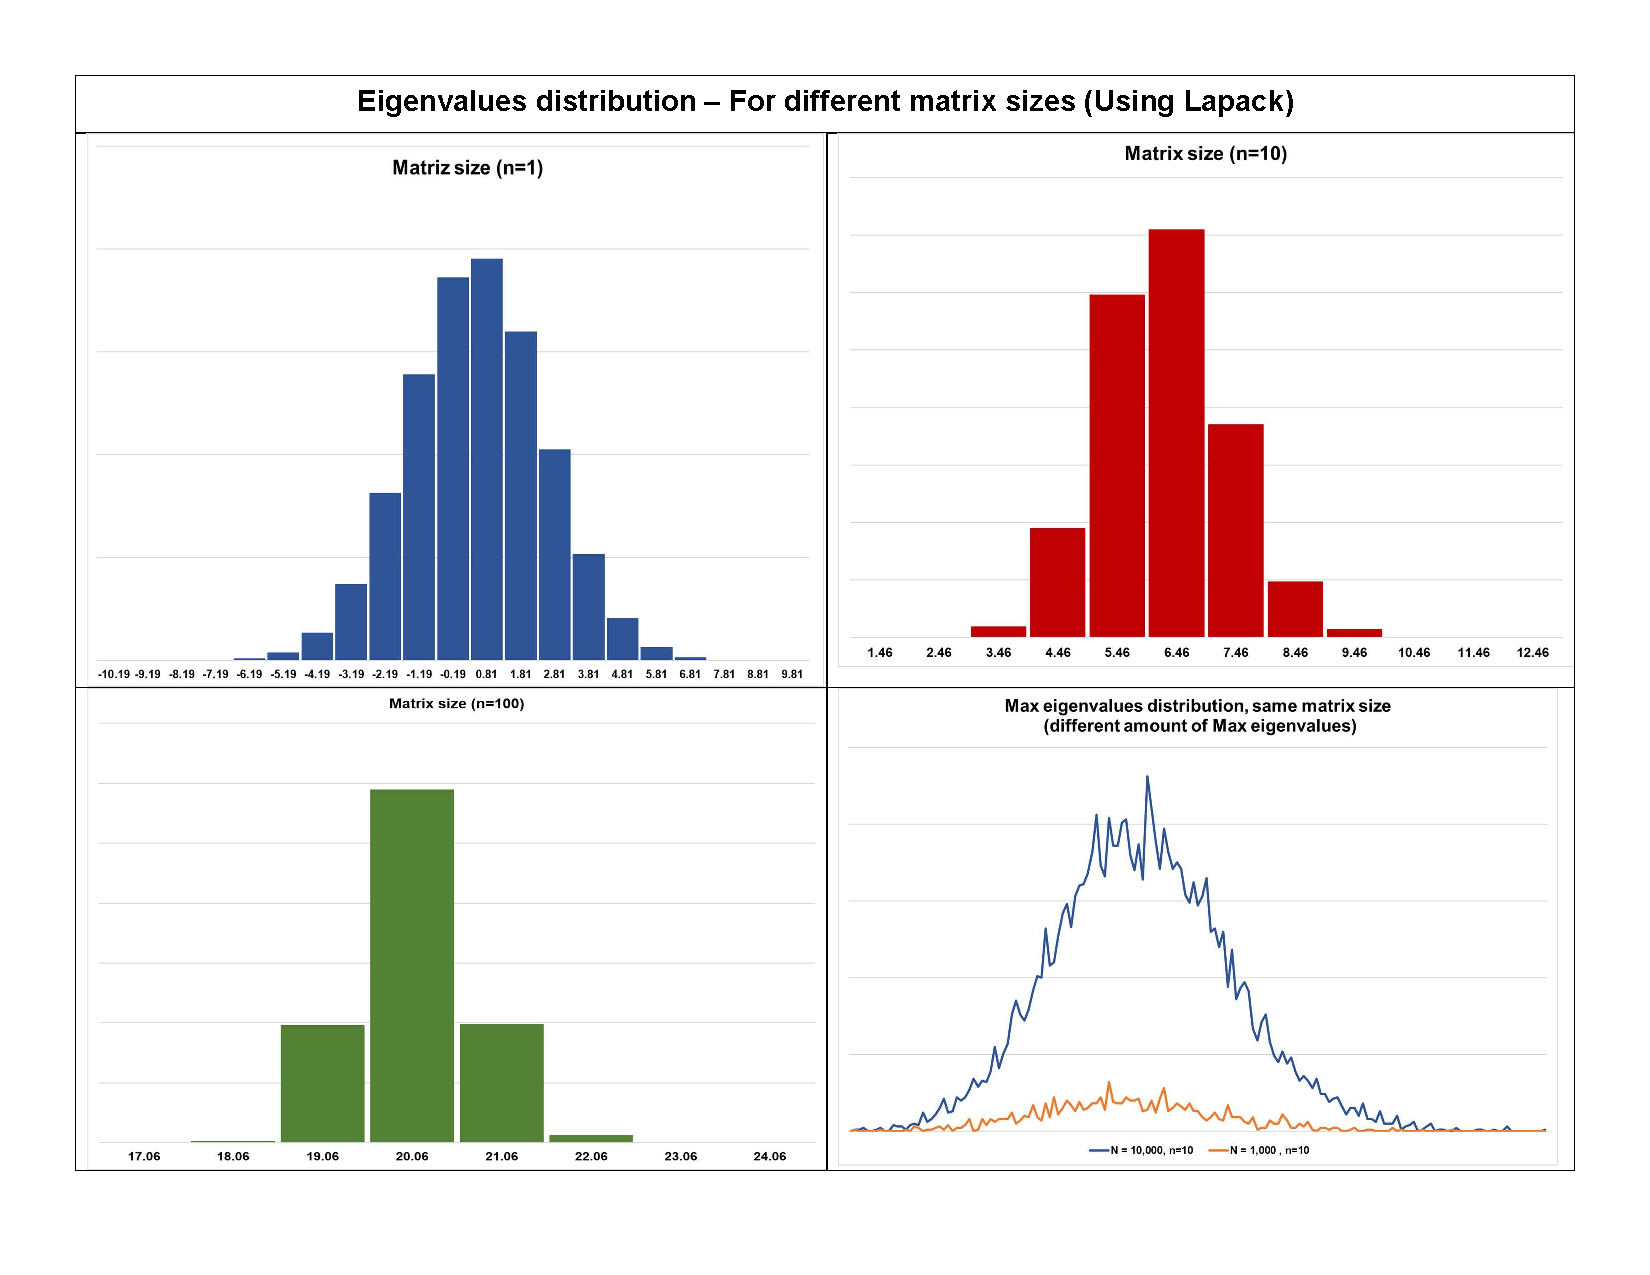
\includegraphics[width=0.75\textwidth]{Figures/D_Lapack.pdf}
		\caption{Distribution of maximum Eigenvalues for computations using LAPACK.}
		\label{fig:2}
	\end{figure}

        In order to identify which distribution could fit in the outputs obtained, a distribution analysis was performed usin IBM-SPSS (Statistical Package Software) and a Komolgorov-Smirnov test was applied to the 10 Eigenvectors. Komolgovorv-Smirnov (KS) is a nonparametric test of the equality of continuous, one-dimensional probability distributions that can be used to compare a sample with a reference probability distribution (one-sample KS test), or to compare two samples (two-sample KS test). The Kolmogorov-Smirnov tests tell us that whether or not a dataset follows a specified distribution by comparing the significance of the data with a given predetermined significance level, which in the present case was taken as 0.05. These results are presented in figure~\ref{fig:3}
        \begin{figure}[h]
		\centering
		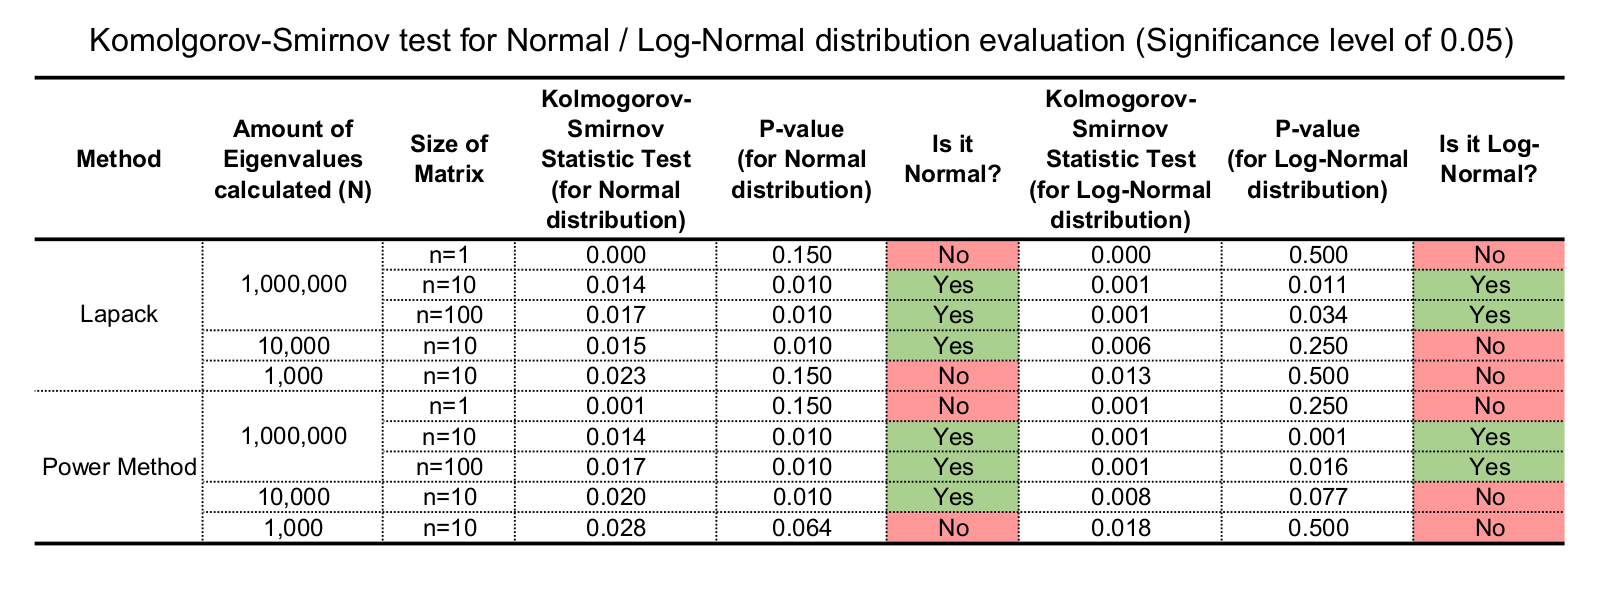
\includegraphics[width=0.95\textwidth]{Figures/tab_test.png}
		\caption{Analysis of the obtained maximum Eigenvalue distributions.}
		\label{fig:3}
	\end{figure}
The results show that the Eigenvalues generally show a log-normal distribution with an increase in the average values as the matrix size was increased.        

The Eigenvalues were computed for different matrix sizes $n$ and different numbers of desired Eigenvalues $N$ using both BLAS and shifted power iterations and the obtained wallclock times were compared. The results are presented below in  figure~\ref{fig:walltime}.
        	\begin{figure}[h]
		\centering
		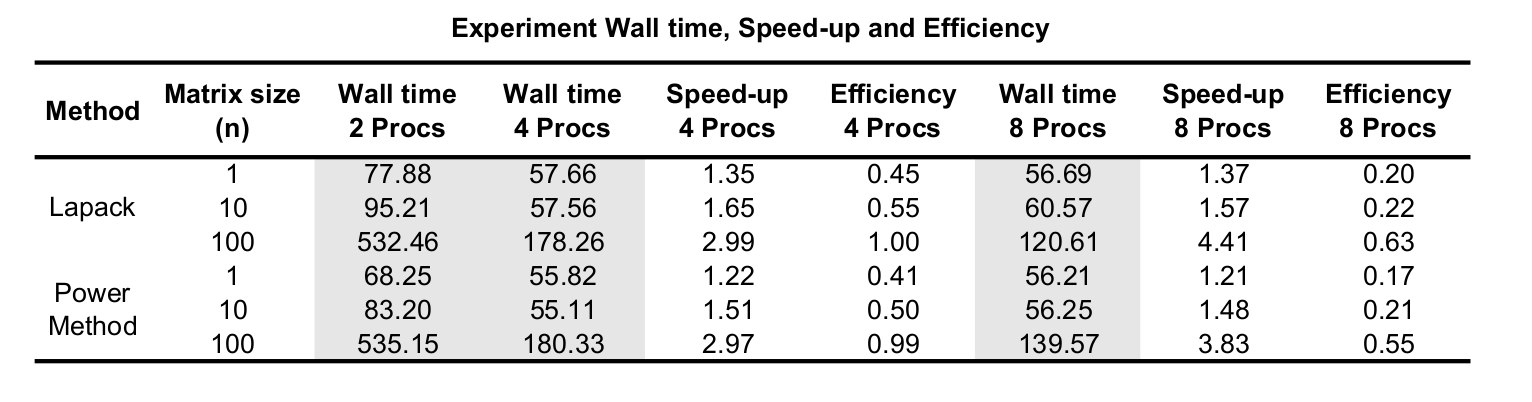
\includegraphics[width=0.95\textwidth]{Figures/eff.png}
		\caption{Wallclock times and performance parameters for different tests.}
		\label{fig:walltime}
	        \end{figure}

 In the available literature, Almeida et al. \cite{Almeida:2013:MEC:2509348.2509354} have shown that wallclock times are inversely proportional to the number of processors and Elenin et al. \cite{Elenin2013EvaluationOM}, have shown that wallclock times as small as those of the order of 0.65s can be obtained. The data shows, as expected, a decrease in wall-clock times as the number of processors is increased from one to three. However, since a further increase means that no physical cores are available and hyperthreads are used, we do not observe any further decrease in wallclock times for an increase in total number of processors beyond 4. Furthermore, the wallclock times of the  power iterations were observed to be smaller than the wallclock times using LAPACK.


\section{Conclusion}
In conclusion, the computational experiments verify the expected outcomes of the study. MPI implementation of the master-slave model resulted in a reduced wallclock times as the number of slaves was increased. The power iteration was quicker than the LAPACK subroutine and the Eigenvalues showed a log-normal distribution with an increase in the average value as the size of the matrix was increased.      

\newpage

\bibliographystyle{ieeetr}
\bibliography{Assignment_4_Parikshit}

\end{document}  
